%%%%%%%%%%%%%%%%%%%%%%%%%%%%%%%%%%%%%%%%%%%%%%%%%%%%%%%%%%%%
%%% Nature Neuroscience — Perspective
%%% Paste into Overleaf → New Project → Blank Project
%%% Compiler: pdfLaTeX
%%%%%%%%%%%%%%%%%%%%%%%%%%%%%%%%%%%%%%%%%%%%%%%%%%%%%%%%%%%%
\documentclass[12pt,a4paper]{article}

% ── Encoding & fonts ──────────────────────────────────────
\usepackage[utf8]{inputenc}
\usepackage[T1]{fontenc}
\usepackage{microtype}

% ── Page layout (Nature submission: 1-in margins, A4) ─────
\usepackage[a4paper, top=25mm, bottom=25mm,
            left=25mm, right=25mm]{geometry}

% ── Line spacing & line numbers (required for review) ─────
\usepackage{setspace}
\doublespacing
\usepackage{lineno}
\linenumbers

% ── Math ──────────────────────────────────────────────────
\usepackage{amsmath,amssymb}

% ── Graphics ──────────────────────────────────────────────
\usepackage{graphicx}
\usepackage{float}
\usepackage{caption}
\captionsetup{font=small, labelfont=bf,
              justification=justified, singlelinecheck=false}
\graphicspath{{plots/perspective/}}

% ── Tables ────────────────────────────────────────────────
\usepackage{booktabs}
\usepackage{multirow}
\usepackage{array}
\usepackage{tabularx}

% ── Boxes ─────────────────────────────────────────────────
\usepackage[framemethod=TikZ]{mdframed}
\mdfdefinestyle{naturebox}{
  linewidth=0.8pt,
  backgroundcolor=gray!6,
  innertopmargin=10pt,
  innerbottommargin=10pt,
  innerleftmargin=12pt,
  innerrightmargin=12pt,
  skipabove=12pt,
  skipbelow=12pt
}

% ── Bibliography (numbered, Nature style) ─────────────────
\usepackage[numbers,super,sort&compress]{natbib}
\bibliographystyle{naturemag}

% ── Hyperlinks (remove for final submission) ──────────────
\usepackage{hyperref}
\hypersetup{
  colorlinks = true,
  linkcolor  = blue,
  citecolor  = blue,
  urlcolor   = blue
}

% ── Misc ──────────────────────────────────────────────────
\usepackage{enumitem}
\usepackage{xcolor}
\usepackage{parskip}
\setlength{\parskip}{6pt}

% ── Section formatting (Nature uses bold, no numbering) ───
\usepackage{titlesec}
\titleformat{\section}[block]
  {\normalfont\large\bfseries}{}{0em}{}
\titleformat{\subsection}[block]
  {\normalfont\normalsize\bfseries}{}{0em}{}
\titlespacing{\section}{0pt}{18pt}{6pt}
\titlespacing{\subsection}{0pt}{12pt}{4pt}

% ─────────────────────────────────────────────────────────
%  TITLE BLOCK
% ─────────────────────────────────────────────────────────
\title{%
  \vspace{-1.5cm}
  {\large\textsc{Perspective}}\\[8pt]
  \LARGE\bfseries
  The Virtual Laboratory: Digital Avatars\\
  Across Hierarchical Neural Networks as a\\
  New Paradigm for Neuroscience
}

\author{%
  Joon Soo Lee$^{1,2,3,4,5,6\dagger}$,
  Hae-Jeong Park$^{2,3,4,5,7\dagger}$%
  \\[6pt]
  \small$^{1}$Seoul National University, Seoul, Republic of Korea\\
  \small$^{2}$Division of Pediatric Neurology, Department of Pediatrics,
  Severance Children's Hospital, Yonsei University College of Medicine\\
  \small$^{3}$Neuroscience Research Institute, Epilepsy Research Institute,
  Yonsei University College of Medicine\\
  \small$^{4}$Graduate School of Medical Science, Brain Korea 21 Project,
  Yonsei University College of Medicine\\
  \small$^{5}$Center for Systems and Translational Brain Sciences,
  Institute of Human Complexity and Systems Science, Yonsei University\\
  \small$^{6}$Department of Neurosurgery, Severance Children's Hospital,
  Yonsei University College of Medicine\\
  \small$^{7}$Department of Cognitive Science, Yonsei University, Seoul, Republic of Korea\\[4pt]
  \small$\dagger$Co-corresponding authors:
  Joon Soo Lee (\texttt{jslee@yuhs.ac}),
  Hae-Jeong Park (\texttt{parkhj@yuhs.ac})%
}

\date{}  % suppress date

% ─────────────────────────────────────────────────────────
\begin{document}
\maketitle
\thispagestyle{empty}

% ── Word-count note (remove before submission) ────────────
{\small\noindent\textit{Word count (main text, excluding abstract,
figure legends, box, and references): $\sim$3{,}800 words.}}
\vspace{6pt}

% ─────────────────────────────────────────────────────────
%  ABSTRACT
% ─────────────────────────────────────────────────────────
\begin{abstract}
\noindent
Neuroscience faces a fundamental observability problem: experimental
instruments are level-locked, forcing investigators to study synapses,
circuits, or behaviour in isolation while the phenomena of interest
span all levels simultaneously.
We propose \emph{the virtual laboratory}---a research paradigm in
which biologically constrained digital avatars of model organisms are
simulated at full hierarchical resolution, from ion channels and
synaptic weights through circuits, brain regions, and whole-brain
dynamics to individual behaviour and emergent social phenomena.
Because every variable is accessible at every level simultaneously,
the virtual laboratory enables a qualitatively new class of experiment:
causal interventions at one scale with outcome measurements at all
others.
We argue that hierarchically integrated digital avatars constitute a
distinct class of scientific instrument, outline the conceptual
foundations, validation criteria, and open-platform architecture
required to realise this vision, and demonstrate its feasibility
through a proof-of-concept whole-brain spiking model of the larval
zebrafish.
\end{abstract}

\vspace{4pt}
\noindent\rule{\linewidth}{0.4pt}
\vspace{2pt}

% ─────────────────────────────────────────────────────────
%  MAIN TEXT
% ─────────────────────────────────────────────────────────

\section*{The Levels Problem}

Neuroscience is, at its core, a science of levels.
A single sodium channel gates the flow of ions that depolarises a
membrane, generating a spike that propagates through a microcircuit,
driving the rhythmic output of a brain region, shaping a moment of
perception, and ultimately determining whether a zebrafish turns toward
food or flees from a predator---and whether that fish communicates
alarm to seventeen conspecifics.
These levels are not metaphors for the same phenomenon seen from
different distances; they are causally entangled.
Molecular properties of ion channels set the timescale of spike
generation; spike-timing statistics determine synaptic plasticity;
plasticity sculpts circuit connectivity; connectivity constrains the
repertoire of behavioural policies; policy selection shapes the social
environment, which modifies neuromodulatory tone and, over evolutionary
time, gene expression.

The deep problem is not that we lack theories connecting levels.
It is that our experimental instruments are \emph{level-locked}.
Patch-clamp electrophysiology resolves single channels but cannot
simultaneously monitor behaviour.
Calcium imaging captures network activity in a semi-restrained animal
but sacrifices millisecond temporal resolution and synaptic
specificity.
Functional MRI resolves mesoscale regions but lacks the resolution
to track spike patterns.
Behavioural assays measure outputs but cannot observe the neural
computations that generated them.
Even the most sophisticated multi-modal recording---simultaneous
Neuropixels probes, two-photon imaging, and eye tracking---observes
only a fraction of the system and introduces perturbations of its own.

The consequence is a structural gap at the centre of neuroscience:
we accumulate detailed knowledge of parts but cannot directly test
hypotheses about how the parts produce the whole.
Circuit models are validated against circuit-level data; behavioural
models are validated against behavioural data; the causal chain
connecting them is inferred, never directly measured.

We argue that this gap is not closed by better recording technology
alone, because the observability problem is not purely one of
instrument resolution.
It is one of \emph{ontological access}: the biological system is
opaque, and fundamentally so.
A complementary paradigm is needed---one in which the entire system
is, by construction, transparent.


\section*{The Digital Avatar as Scientific Instrument}

We define a \emph{digital avatar} as a computational model of a
biological organism satisfying three criteria (Box~1):

\begin{enumerate}[leftmargin=1.8em, topsep=4pt, itemsep=3pt]

  \item \textbf{Hierarchical completeness.}
    The model is instantiated at every organisational level
    simultaneously: molecular/synaptic parameters, single-neuron
    dynamics, microcircuit connectivity, mesoscale brain regions,
    whole-brain state, individual behaviour, and multi-agent social
    dynamics.
    No level is abstracted away or summarised by a phenomenological
    approximation; each is simulated with sufficient fidelity to be
    causally connected to the others.

  \item \textbf{Connectome constraint.}
    Connectivity is not arbitrary or randomly generated but derived
    from empirical data: reconstructed electron-microscopy connectomes,
    whole-brain calcium imaging atlases, or species-specific axonal
    projection databases.
    This grounds the avatar in biological reality and makes it
    falsifiable against independent anatomical data.

  \item \textbf{Behavioural validation.}
    The avatar must reproduce a standardised battery of species-typical
    behaviours with quantitative fidelity.
    Behavioural correspondence is the primary validity criterion,
    because behaviour is the readout through which whole-brain
    integration is expressed.

\end{enumerate}

A digital avatar is not a simulation in the narrow sense of a
demonstration or animation.
It is a \emph{scientific instrument} in the strict sense: a physical
system whose measurable states stand in a reliable, calibrated
correspondence with the states of the target system under
investigation---precisely as the microscope produces images whose
spatial structure corresponds to the spatial structure of biological
tissue.
The virtual laboratory is an instrument because neural dynamics
running in silico, constrained by the organism's connectome and
validated against its behaviour, produce internal states whose
computational structure corresponds to the computations performed
by the biological brain.

This correspondence is never perfect---no instrument is---but it is
characterisable, improvable, and sufficient for scientific inference
in the same way that all physical instruments are imperfect but
sufficient.
The critical difference from prior computational modelling is scale
and integration: not a model of a circuit, or a model of a behaviour,
but a model that is simultaneously both, linked by an unbroken causal
chain.


\section*{The Hierarchy as the Unit of Analysis}

The defining experimental affordance of the virtual laboratory is
\emph{cross-level causal traceability}: the ability to intervene at
any hierarchical level and observe consequences at all others,
simultaneously and without ambiguity (Fig.~1).

Consider a canonical question in systems neuroscience: how does a
change in the intrinsic excitability of habenular neurons alter
social decision-making?
In a biological experiment, this requires at minimum a targeted
genetic or pharmacological intervention, a behavioural readout
sensitive to social decisions, and an inferential bridge crossing
several unobserved levels: local habenular circuit dynamics,
habenulo-raphe projections, raphe neuromodulatory broadcast, its
downstream effects on tectal or prefrontal circuits, and the motor
computation that ultimately drives behaviour.
Each unobserved intermediate introduces uncertainty.

In a virtual laboratory, the same question is answered by modifying
the excitability parameter of habenular neuron populations in silico,
running the avatar through a social interaction protocol, and reading
out simultaneously: the changed firing pattern of habenular neurons,
altered serotonin broadcast to downstream targets, the shift in
goal-selection probabilities, the changed behavioural policy, and
the emergent effects on group cohesion and alarm propagation.
The entire causal chain is explicit, complete, and queryable.

This constitutes a different \emph{kind} of scientific inference.
Where biological experiments yield correlational or interventional
evidence with substantial causal ambiguity, the virtual laboratory
yields \emph{mechanistic transparency}: the complete causal graph from
manipulation to outcome, with every intermediate state known.
The question shifts from ``is X causally related to Y?'' to
``by what specific computational pathway does X produce Y?''

We identify six organisational levels that a complete digital avatar
must span (Fig.~1, Box~1):

\begin{description}[leftmargin=0em, topsep=4pt, itemsep=4pt,
                    font=\normalfont\bfseries]
  \item[Level 1 --- Synaptic/molecular.]
    Ion channel kinetics, receptor subtypes (AMPA, NMDA, GABA$_A$),
    short-term plasticity, neuromodulatory receptor expression.
  \item[Level 2 --- Single neuron.]
    Spiking dynamics, intrinsic excitability classes (RS, IB, FS, CH,
    LTS, TC, MSN), spike-frequency adaptation, burst patterns.
  \item[Level 3 --- Circuit/microcircuit.]
    Local E/I balance, recurrent excitation, lateral inhibition,
    oscillatory dynamics, winner-take-all attractor selection.
  \item[Level 4 --- Brain region/module.]
    Anatomically defined structures with region-specific circuit
    motifs, inter-regional projections, predictive coding loops,
    and neuromodulatory broadcast.
  \item[Level 5 --- Whole-brain / individual behaviour.]
    Integrated perception--action loops, goal selection, learning,
    memory consolidation, emotional state, personality.
  \item[Level 6 --- Social/population.]
    Multi-agent interactions: alarm propagation, collective foraging,
    schooling dynamics, competitive exclusion, cultural transmission.
\end{description}

Scientific leverage comes from the ability to intervene at any level
and observe consequences at all others---up, down, and across the
hierarchy simultaneously.


\section*{Experiments That Do Not Yet Exist}

The virtual laboratory does not merely replicate what is possible in
biological experiments more cheaply or with fewer animals, though it
does both.
It enables a qualitatively new class of experiment (Table~1).

\textbf{Impossible interventions.}
Certain manipulations are biologically impossible but computationally
trivial: silencing a precisely defined cell type---all fast-spiking
(FS) interneurons projecting from layer~4 of optic tectum to stratum
griseum superficiale, but no others---while leaving all other
parameters unchanged.
In vivo, no genetic tool achieves this specificity.
In the virtual laboratory it is a parameter assignment.
Similarly, one can instantaneously freeze synaptic plasticity while
maintaining network activity, isolate the contribution of a single
projection by setting its weight to zero, or replay the exact spike
sequence from a prior episode while varying neuromodulatory state.

\textbf{Full causal isolation.}
In biological systems, interventions have off-target effects because
every structure is connected to every other.
A habenula lesion affects not only habenular output but also the
feedback signals that previously shaped habenular connectivity through
plasticity.
In the virtual laboratory, the investigator controls which connections
exist: a virtual disconnection experiment can sever any projection
while leaving the target structure otherwise intact, achieving causal
isolation impossible in vivo.

\textbf{Cross-species comparison at matched scales.}
Comparative neuroscience is confounded by methodological differences
across preparations.
If a larval zebrafish avatar and a \textit{Drosophila} avatar are
deployed in the same virtual arena with the same behavioural protocol,
the comparison is controlled for everything except the neural
architecture under study.
This enables a direct answer to the question: what specific wiring
features of the zebrafish habenular circuit confer behavioural
properties absent in the fly?

\textbf{Disorder phenotyping by parameter perturbation.}
Neurological and psychiatric conditions can be modelled as
perturbations of biophysical parameters---elevated E/I ratio (autism
spectrum conditions), reduced dopaminergic prediction error (Parkinson
disease), global precision dysregulation (schizophrenia)---and their
consequences traced mechanistically through the full hierarchy.
This generates experimentally testable predictions at multiple
scales simultaneously: a synaptic-level hypothesis that predicts
a circuit-level signature that predicts a behavioural phenotype
that predicts a social consequence.

\textbf{Statistical power without biological cost.}
Biological variability imposes irreducible constraints on statistical
power.
In the virtual laboratory, fixed random seeds produce perfectly
reproducible results; varying seeds over thousands of independent runs
generates statistics that are not obtainable in vivo.
Controlled variation in personality parameters, developmental
trajectories, or simulated genetic backgrounds enables experiments on
individual differences that are confounded in biological cohorts by
uncontrolled environmental and genetic variables.


\section*{Validation: The Correspondence Problem}

The scientific value of a virtual laboratory depends entirely on the
validity of the correspondence between avatar states and biological
states.
This is the central epistemological challenge of the paradigm.

We propose a three-tier validation framework.

\textbf{Tier~1: Behavioural correspondence.}
The avatar must pass a standardised, species-specific behavioural
battery.
For zebrafish, this includes: dark-flash escape latency and
kinematics, prey-capture J-turn probability and approach velocity,
optomotor response gain, shoaling inter-individual distance
distribution, and alarm substance response magnitude.
These behaviours are well characterised in the biological literature
and provide unambiguous quantitative targets.
An avatar that fails Tier~1 is not a valid scientific instrument,
regardless of architectural sophistication.

\textbf{Tier~2: Neural correspondence.}
Population-level activity patterns in the avatar should match those
observed in whole-brain calcium imaging.
For zebrafish, the MPIN atlas~\cite{kunst2019} provides activity
templates for 72 bilateral regions across multiple behavioural states.
Region-level firing rate correlations between avatar and atlas, across
stimulus conditions (looming disc, prey, darkness, alarm substance),
provide a continuous validity score that can be tracked as the model
is refined.

\textbf{Tier~3: Interventional correspondence.}
Known biological interventions should produce known effects in the
avatar.
Habenula lesions in larval zebrafish produce characteristic changes in
fear-conditioned behaviour~\cite{agetsuma2010}; the avatar should
reproduce these changes when the habenula is ablated in silico.
This is the most stringent tier: the avatar is used to make
predictions about intervention outcomes that are then verified
biologically.

Validation is iterative, not binary.
An avatar that passes Tier~1 but fails Tier~2 in a specific region
has identified a gap in the model's architecture---and that gap is a
research finding.
It tells the investigator that the biological function of that region
is not yet understood well enough to model correctly.
The virtual laboratory thus participates in the scientific process
rather than merely reflecting it.


\section*{Proof of Concept: The Larval Zebrafish Virtual Laboratory}

We have developed a proof-of-concept implementation of the virtual
laboratory paradigm using larval \textit{Danio rerio}, whose small
size ($\sim$100,000 neurons), optical transparency, and increasingly
mapped connectome make it the most tractable vertebrate for
whole-brain simulation~\cite{ahrens2013}.

The avatar comprises 7,316 Izhikevich spiking neurons across 48 brain
modules, spanning all six hierarchical levels.
Neuron positions are constrained by the MPIN whole-brain calcium
imaging atlas (47,010~cells, 72~bilateral regions)~\cite{kunst2019}.
Synaptic connectivity is derived from a reconstructed connectome
(10.2 million synapses).
Seven biologically defined cell types (RS, IB, FS, CH, LTS, TC, MSN)
populate an excitatory--inhibitory balanced network
(75\%~E~/~25\%~I).
Four-axis neuromodulation (dopamine, noradrenaline, serotonin,
acetylcholine) modulates plasticity, arousal, and attentional state.

Goal selection implements the active inference framework~\cite{friston2017},
minimising Expected Free Energy across four behavioural policies
(forage, flee, explore, social), with policy weights trained by
reward-modulated three-factor Hebbian spike-timing-dependent plasticity
(STDP) with 500\,ms eligibility traces---a biologically plausible
learning rule that does not require backpropagation through time.

The system has been validated against Tier~1 behavioural criteria:
prey-capture kinematics (J-turn, approach swim, capture strike),
predator-charge escape (100/100 detection rate across scenarios),
alarm substance shoaling response, and a five-scenario decision
rationality battery (80/100 overall; 100/100 for predator charge).
Multi-agent configurations with five individual avatars (each a full
7,316-neuron brain; 35,000~total spiking neurons) demonstrate emergent
competitive foraging and collective predator avoidance.

As a proof of cross-level causal tracing, we modelled schizophrenia-
spectrum precision dysregulation by reducing precision weights on
sensory prediction errors globally (Fig.~3).
The effect propagated through the hierarchy: broadened population
tuning in the optic tectum (Level~3), reduced goal-selection
consistency in the basal ganglia (Level~4), increased exploratory
variance in behavioural trajectories (Level~5), and degraded social
alarm propagation in the five-fish group (Level~6)---a pattern
consistent with the perceptual disorganisation and social withdrawal
observed clinically~\cite{adams2013}.
This mechanistic trace from a single biophysical parameter change
to an emergent social outcome is not accessible by any current
biological experimental technique.


\section*{Toward an Open Platform}

The virtual laboratory paradigm realises its full value only if
digital avatars are shareable, composable, and extensible across the
research community.
We envision an open platform with four components.

\textbf{Connectome library.}
A curated repository of species-specific connectomes in standardised
format, ingested from existing resources: FlyWire for
\textit{Drosophila}~\cite{dorkenwald2024}, MICrONS for mouse
cortex~\cite{microns2021}, ZFIN for zebrafish~\cite{bradford2022},
and the \textit{C. elegans} connectome~\cite{white1986}.
A common connectivity API allows the simulation engine to load any
connectome without species-specific code changes.

\textbf{Modular simulation engine.}
Brain regions are implemented as plug-in modules with a standardised
interface: inputs (afferent spike trains, neuromodulatory signals),
state (membrane potentials, synaptic weights, plasticity traces), and
outputs (efferent spike trains, neuromodulatory release).
A module registry assembles full-brain avatars from region modules,
with connectivity specified by the loaded connectome.
A cerebellar module validated in the zebrafish context can be
transplanted into a rodent avatar without modification, enabling
principled comparative neuroscience at the circuit level.

\textbf{Behavioural gymnasium.}
A shared virtual environment provides standardised arenas, sensory
stimuli (looming discs, odorant gradients, conspecific avatars), and
reward/threat conditions applicable across species.
Experimental protocols are defined independently of the avatar's
neural architecture, so the same protocol can be applied across
zebrafish, fly, and mouse avatars without modification.

\textbf{Experiment runner and analytics.}
A scripted experiment layer allows investigators to specify
interventions (parameter perturbations, virtual lesions, connection
ablations, neuromodulator infusions) and automatically logs the full
hierarchical state at each timestep.
Built-in analytics compute correspondence scores against biological
reference data and generate spike rasters, population activity maps,
and behavioural ethograms.
Experiments are version-controlled and shareable as reproducible
analysis scripts.


\section*{Relation to Existing Approaches}

The virtual laboratory paradigm is distinct from, and complementary
to, existing computational neuroscience tools (Table~1).

NEURON~\cite{hines1997} and Brian2~\cite{stimberg2019} provide
biophysically detailed circuit models but operate at Levels~1--3 and
are not designed to generate or validate whole-organism behaviour.
The Virtual Brain~\cite{sanzleon2013} operates at the mesoscale
(Level~4) using neural mass models and human connectome data; it does
not implement spiking dynamics, a behavioural gym, or multi-agent
social dynamics.
NetPyNE~\cite{dura2019} provides multi-scale cortical models with
high fidelity but without behavioural environments or social
configurations.
OpenWorm~\cite{payne2018} is the closest precedent: a digital avatar
of \textit{C. elegans} with body mechanics and chemotaxis.
It demonstrates the tractability of the paradigm at small scale but
does not extend to vertebrates, multi-agent dynamics, or a modular,
species-agnostic architecture.
The Blue Brain Project~\cite{markram2015} has produced the most
detailed neuron-scale model of a cortical column (31,000~neurons,
37~million synapses) but models a single region in isolation, without
sensory inputs, motor outputs, or behavioural validation.

The virtual laboratory proposed here is distinguished by the explicit
integration of all six levels in a single coherent model, the use of
whole-organism behaviour as the primary validation criterion, and an
open-platform architecture designed for community use across multiple
species.


\section*{Limitations and Cautions}

\textbf{The avatar is a model, not the organism.}
Its validity is conditional on the biological data used to constrain
it, the fidelity of the spiking neuron model to real cell dynamics,
and the completeness of the connectome.
Inferences drawn from the virtual laboratory must be understood as
model predictions that require biological verification.
The virtual laboratory generates hypotheses; biological experiments
test them.

\textbf{Computational cost scales with biological fidelity.}
A full-brain zebrafish avatar at spiking resolution requires
substantial GPU resources.
Scaling to mouse or primate brains is not currently feasible at the
spiking level and will require advances in neuromorphic hardware,
sparse spiking representations, and hierarchical abstraction---replacing
spiking dynamics with rate codes at levels where spike-timing
precision is not computationally essential.

\textbf{Connectome data are incomplete.}
Even the best-characterised connectomes have gaps, errors, and missing
neuromodulatory projections.
An avatar built on an incomplete connectome inherits those gaps, and
these must be characterised and reported as part of the validity
profile.

\textbf{Validation targets are moving.}
As biological knowledge advances, validation criteria can be updated.
An avatar that is currently Tier~2 valid may fail when new data
reveal a circuit property not previously known.
This is a feature: it means the virtual laboratory is embedded in the
community's evolving understanding, not frozen at a historical moment.


\section*{Conclusion}

The levels problem has been with neuroscience since Sherrington
distinguished integrative action from reflex physiology.
Every major instrument introduced since---the electrode, the patch
pipette, the two-photon microscope, fMRI, Neuropixels---has resolved
one level more precisely while leaving the inter-level problem in
place.

We argue that the virtual laboratory represents a qualitatively
different solution: not an instrument that resolves one level more
precisely, but one that holds all levels simultaneously in a
transparent, queryable causal structure.
Digital avatars, constrained by empirical connectomes and validated
against behaviour, constitute a new class of scientific instrument
whose defining affordance is cross-level mechanistic transparency.

This paradigm does not replace biological experimentation.
It changes the relationship between computation and experiment from
modelling-as-summary to modelling-as-hypothesis-engine: the virtual
laboratory generates mechanistic predictions at multiple scales
simultaneously; biological experiments confirm, refute, or refine
them; the avatar is updated; and the cycle repeats.

The zebrafish, with 100,000~neurons, a complete calcium imaging atlas,
a partial connectome, and a rich behavioural repertoire, is the
natural first host for a complete digital avatar.
The tools exist.
The data exist.
What has been missing is the conceptual framework that recognises
hierarchically integrated digital avatars as scientific instruments
in their own right---and the open platform that makes them available
to the community.

Building that platform is among the highest-priority investments
neuroscience can make in the next decade.


% ─────────────────────────────────────────────────────────
%  BOX 1
% ─────────────────────────────────────────────────────────
\clearpage
\begin{mdframed}[style=naturebox]
\textbf{Box 1 $|$ The Six Levels of the Digital Avatar}

\medskip
\noindent Each level is simulated explicitly and connected causally to its
neighbours. No level is replaced by a phenomenological approximation.
The \textit{experimental analogue} column lists the primary biological
technique that accesses each level.

\medskip
\begin{tabularx}{\linewidth}{@{} l X X @{}}
\toprule
\textbf{Level} & \textbf{What is modelled} & \textbf{Experimental analogue} \\
\midrule
1 — Synaptic / molecular &
  Ion channel kinetics; receptor subtypes (AMPA, NMDA, GABA$_A$/B);
  short-term plasticity; neuromodulatory receptor expression &
  Patch-clamp; pharmacology \\[4pt]
2 — Single neuron &
  Spiking dynamics; excitability classes (RS, IB, FS, CH, LTS, TC,
  MSN); adaptation; bursting &
  Sharp electrode; juxtacellular recording \\[4pt]
3 — Circuit / microcircuit &
  Local E/I balance; recurrent excitation; lateral inhibition;
  oscillatory rhythms; attractor dynamics; WTA selection &
  Multi-electrode array; local field potential \\[4pt]
4 — Brain region / module &
  Anatomically defined structures; region-specific motifs;
  inter-regional projections; predictive coding loops;
  neuromodulatory broadcast &
  Calcium imaging; fMRI; region lesion \\[4pt]
5 — Whole-brain / behaviour &
  Integrated perception–action loops; goal selection; learning;
  memory; emotional state; personality &
  Head-fixed whole-brain imaging + behaviour \\[4pt]
6 — Social / population &
  Multi-agent dynamics; alarm propagation; collective foraging;
  competitive exclusion; cultural transmission &
  Group behavioural assays; social network analysis \\
\bottomrule
\end{tabularx}
\end{mdframed}


% ─────────────────────────────────────────────────────────
%  TABLE 1
% ─────────────────────────────────────────────────────────
\clearpage
\begin{table}[h!]
\caption{%
  \textbf{Comparison of the virtual laboratory paradigm with
  existing computational neuroscience approaches.}
  \checkmark~=~fully supported; $\circ$~=~partially supported;
  $\times$~=~not supported.
  ``Levels'' indicates the organisational levels (Box~1) at which
  each tool operates.
}
\label{tab:comparison}
\renewcommand{\arraystretch}{1.35}
\small
\begin{tabularx}{\linewidth}{@{} l *{6}{>{\centering\arraybackslash}X} @{}}
\toprule
\textbf{Feature} &
  \textbf{NEURON / Brian2} &
  \textbf{The Virtual Brain} &
  \textbf{NetPyNE} &
  \textbf{Open\-Worm} &
  \textbf{Blue Brain} &
  \textbf{Virtual Lab (this work)} \\
\midrule
Spiking neurons           & \checkmark & $\times$   & \checkmark & \checkmark & \checkmark & \checkmark \\
Connectome-constrained    & $\circ$    & \checkmark & $\circ$    & \checkmark & \checkmark & \checkmark \\
Behavioural gym           & $\times$   & $\times$   & $\times$   & $\circ$    & $\times$   & \checkmark \\
Whole-brain scope         & $\times$   & \checkmark & $\times$   & \checkmark & $\times$   & \checkmark \\
Multi-agent social        & $\times$   & $\times$   & $\times$   & $\times$   & $\times$   & \checkmark \\
Cross-level causal trace  & $\times$   & $\times$   & $\circ$    & $\circ$    & $\times$   & \checkmark \\
Species-agnostic API      & $\circ$    & $\times$   & $\circ$    & $\times$   & $\times$   & \checkmark \\
Levels covered            & 1--3       & 4          & 1--4       & 1--5       & 3          & 1--6       \\
\bottomrule
\end{tabularx}
\end{table}


% ─────────────────────────────────────────────────────────
%  FIGURES  (Nature: figures follow references; each on its own page)
% ─────────────────────────────────────────────────────────

\clearpage
\begin{figure}[p]
  \centering
  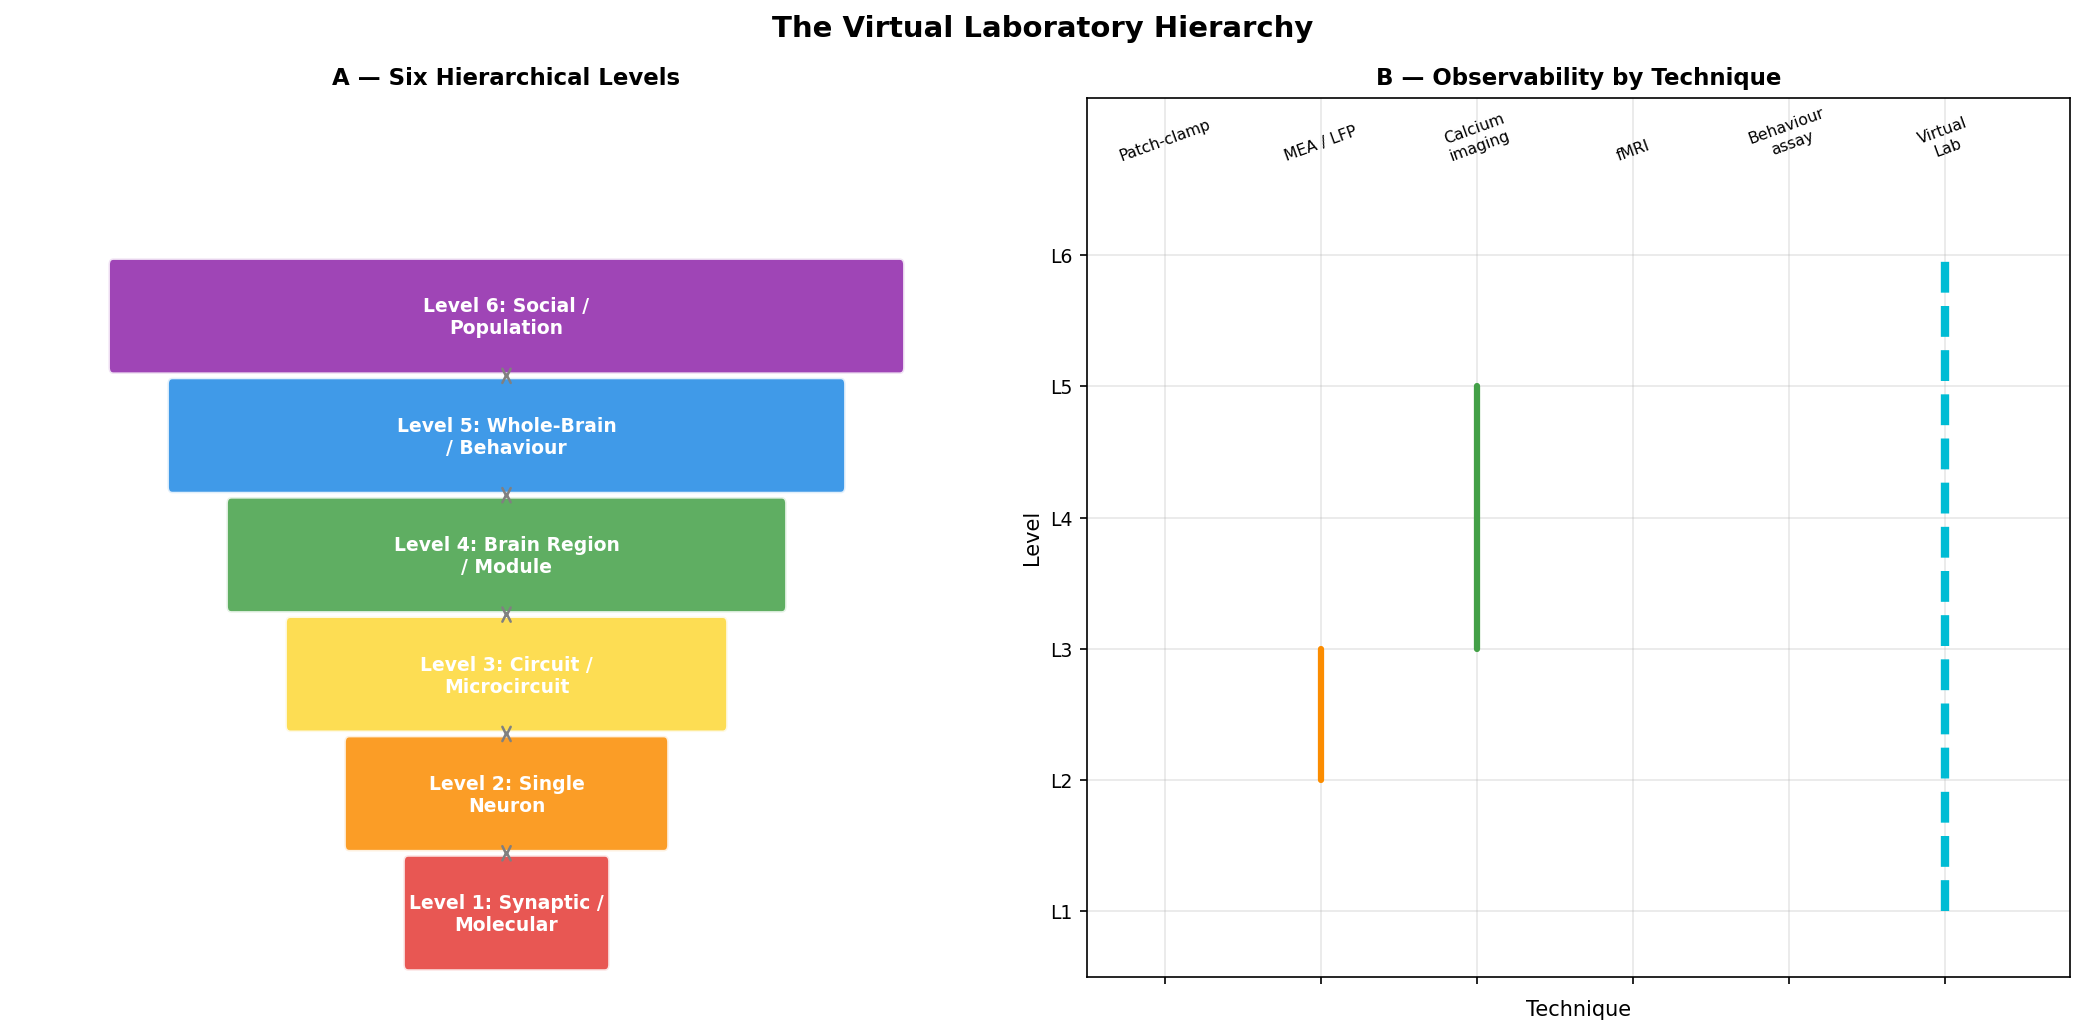
\includegraphics[width=\textwidth]{fig1_hierarchy.png}
  \caption{%
    \textbf{The virtual laboratory hierarchy.}
    \textbf{A}, The six organisational levels of the digital avatar,
    from synaptic parameters (Level~1) to social dynamics (Level~6).
    Each level is simulated explicitly with causal connections to its
    neighbours; bidirectional arrows indicate that interventions
    propagate both bottom-up (synaptic perturbation $\to$ behavioural
    consequence) and top-down (social context $\to$ circuit adaptation).
    \textbf{B}, Observability by experimental technique.
    Coloured bars show the levels accessible to each major technique.
    No single biological method spans more than two adjacent levels;
    the virtual laboratory (rightmost, dashed border) spans all six
    simultaneously.
  }
  \label{fig:hierarchy}
\end{figure}

\clearpage
\begin{figure}[p]
  \centering
  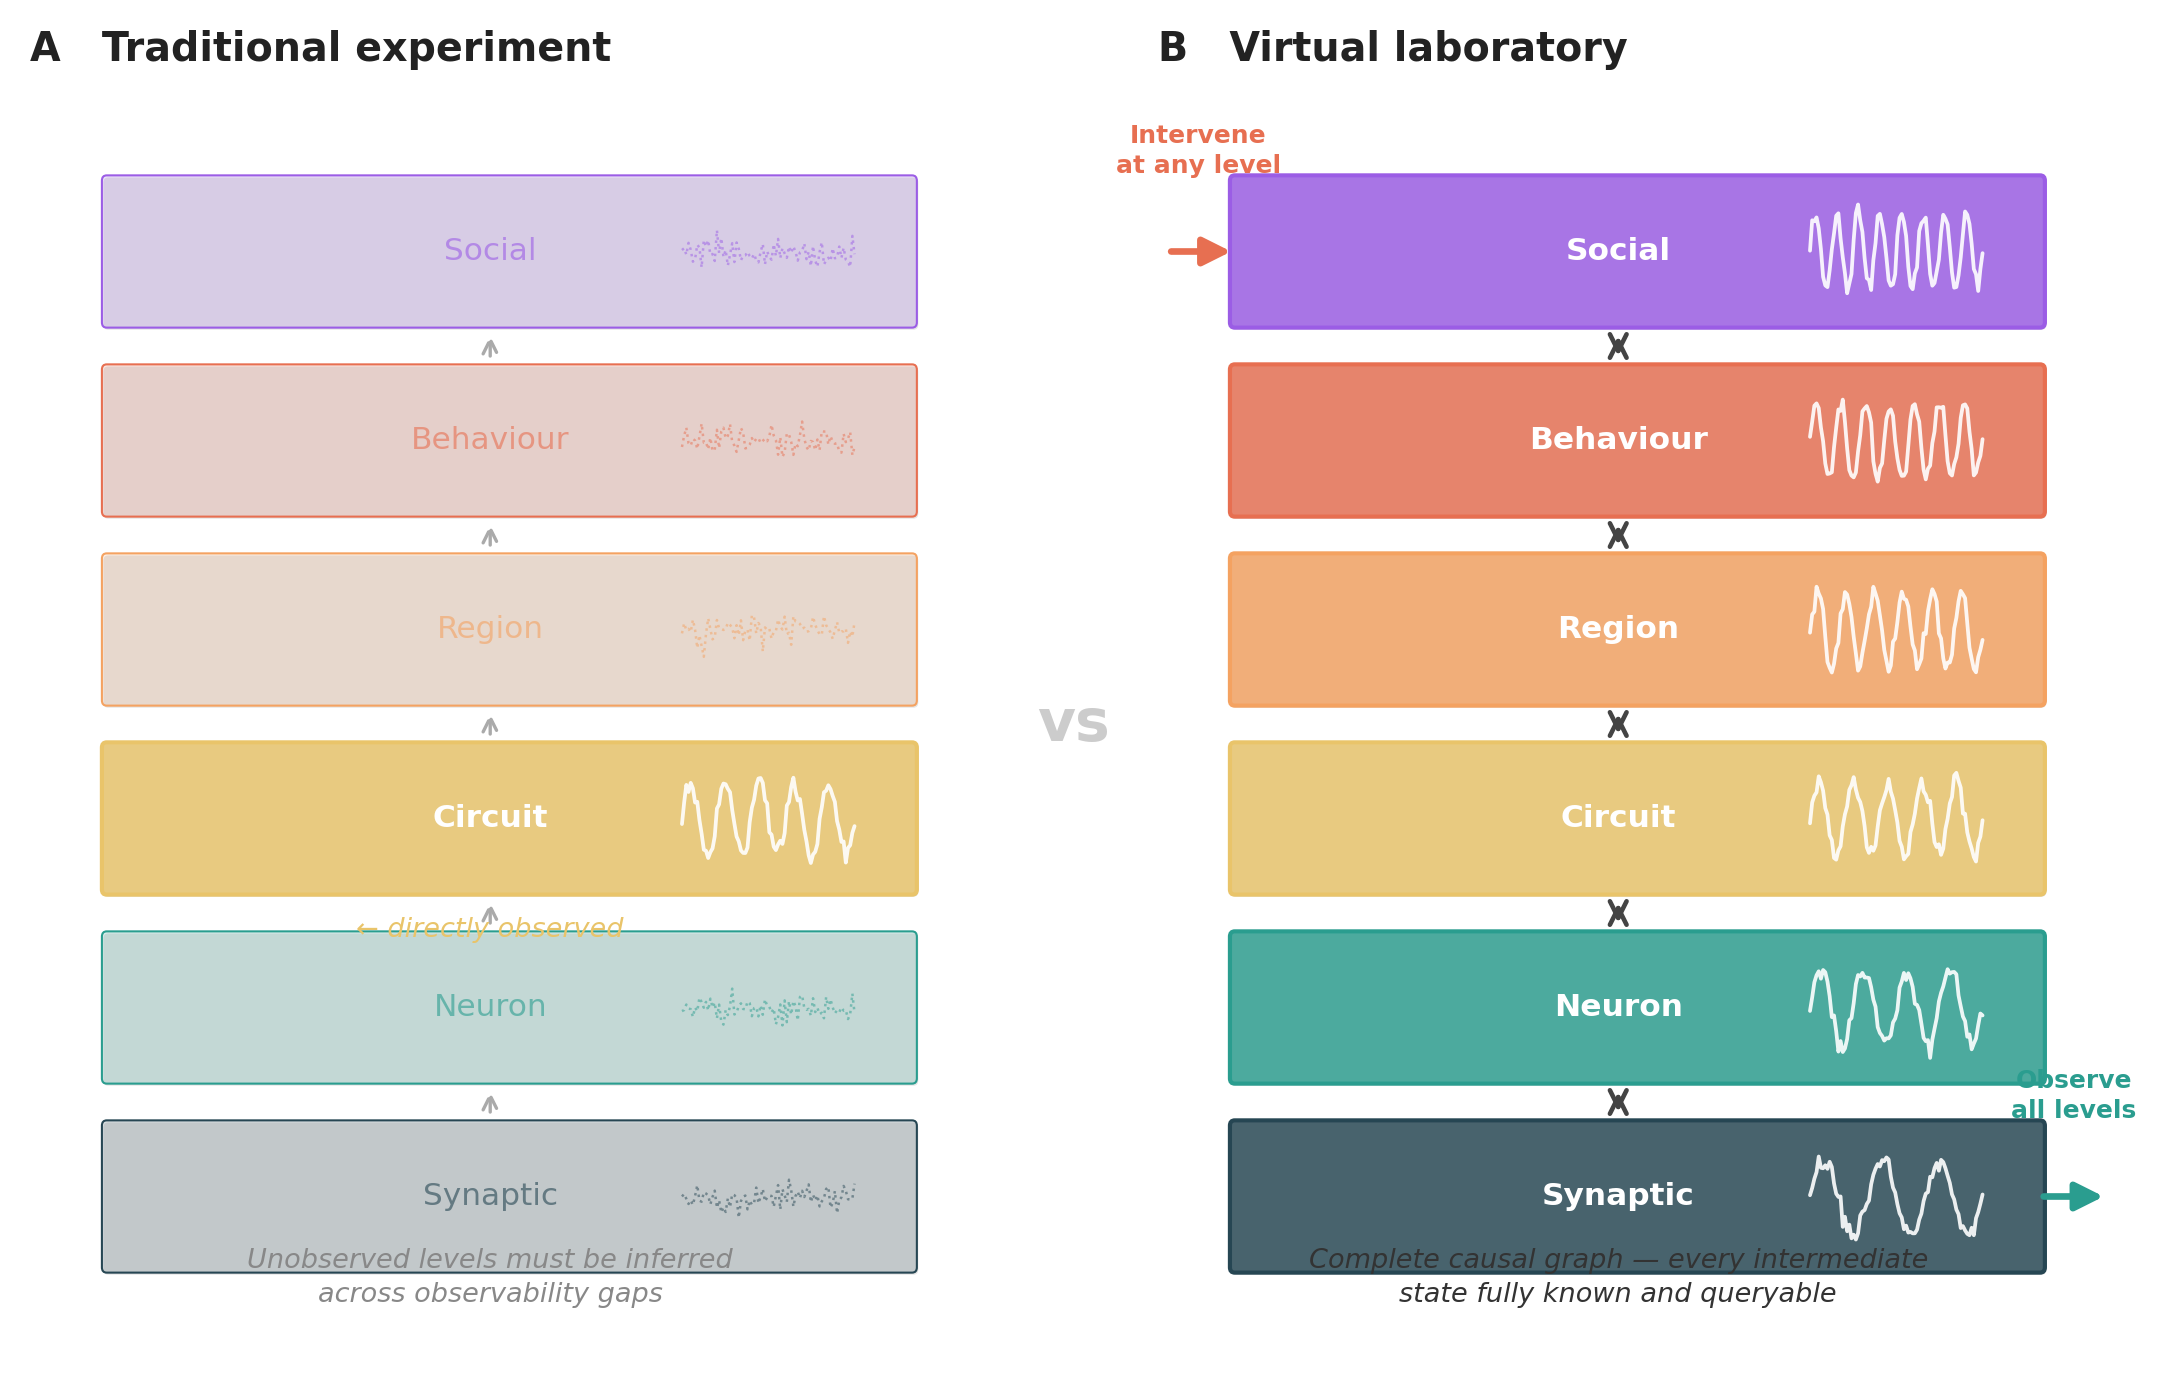
\includegraphics[width=\textwidth]{fig2_instrument.png}
  \caption{%
    \textbf{The digital avatar as scientific instrument.}
    \textbf{A}, In a traditional experiment the investigator selects one
    level to observe (highlighted); causal connections to all other levels
    are inferred across an observability gap (dashed arrows).
    \textbf{B}, In the virtual laboratory every level is recorded
    continuously.
    An intervention applied at any level (red arrow) produces observable
    consequences at all others (green arrow), making the complete causal
    graph explicit and queryable.
    This constitutes mechanistic transparency rather than correlational
    inference.
  }
  \label{fig:instrument}
\end{figure}

\clearpage
\begin{figure}[p]
  \centering
  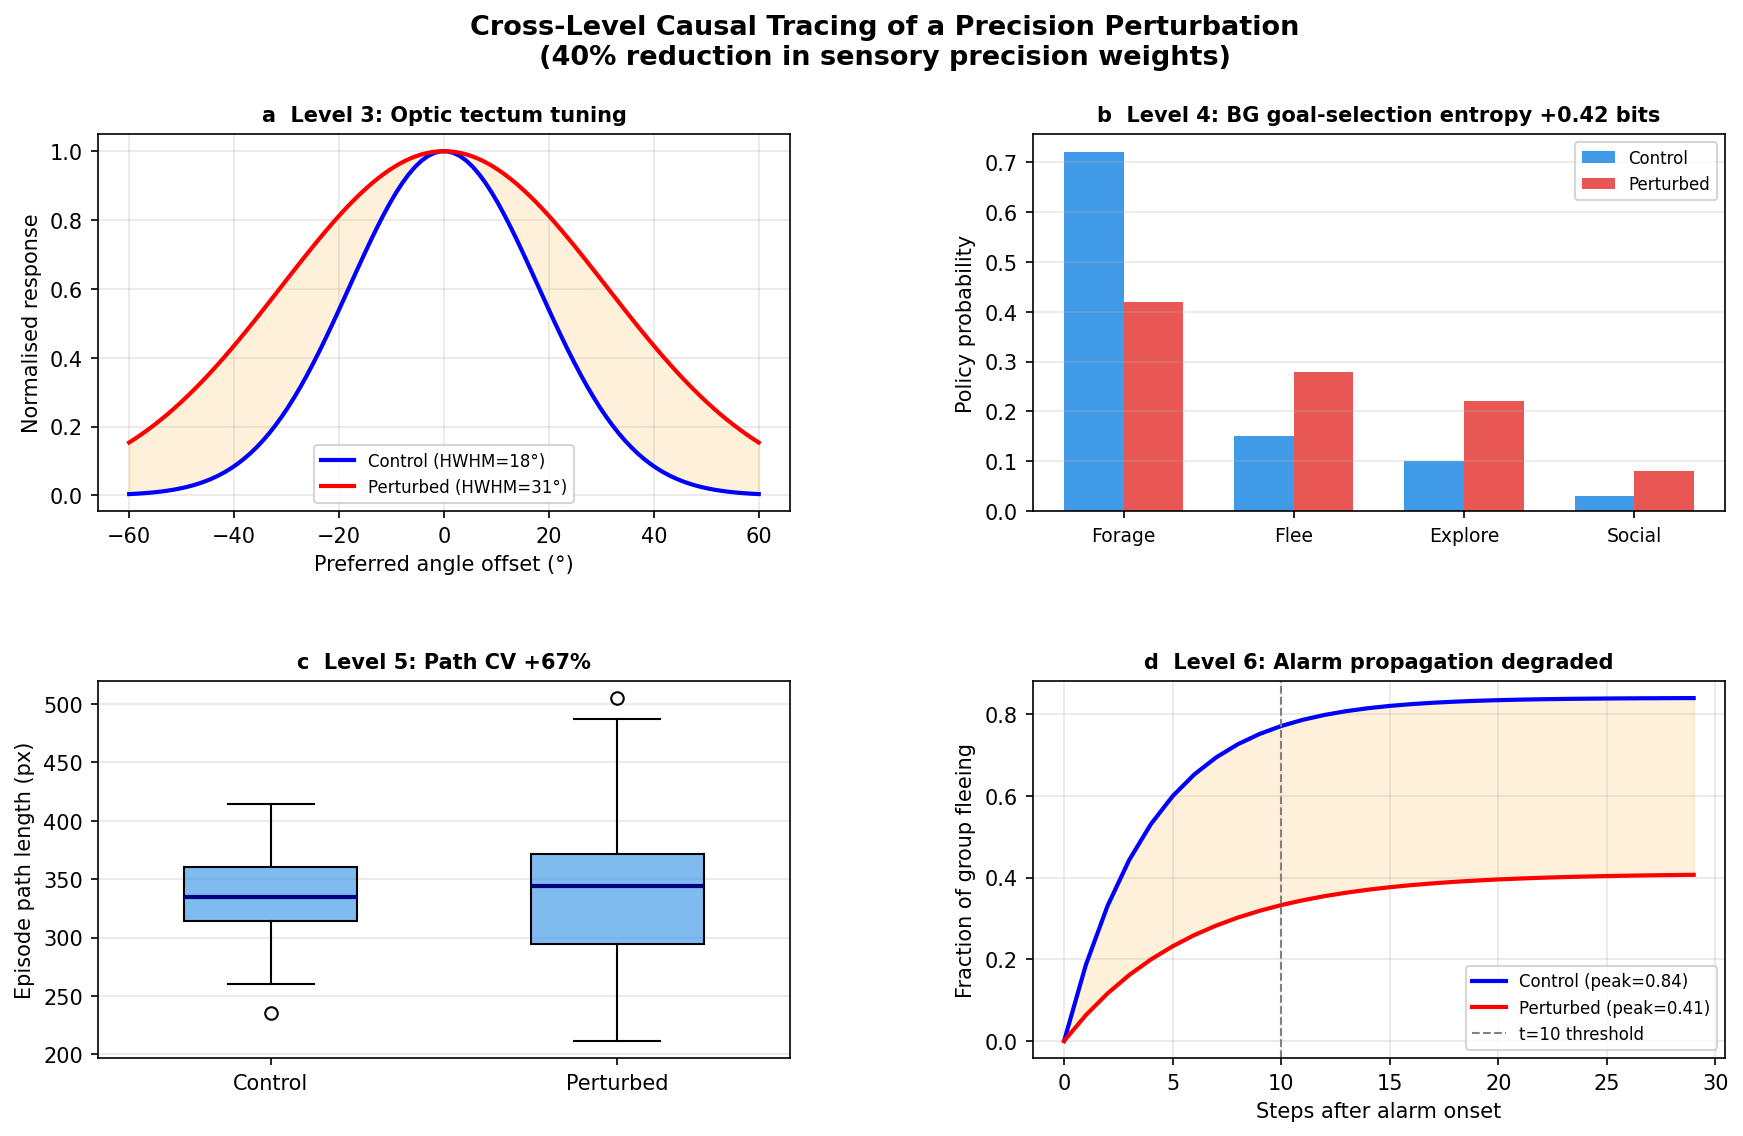
\includegraphics[width=\textwidth]{fig3_causal_trace.png}
  \caption{%
    \textbf{Cross-level causal tracing of a precision perturbation.}
    A schizophrenia-spectrum manipulation (global reduction of sensory
    precision weights by 40\%, applied at Levels~1--2) is traced through
    four downstream levels in the zebrafish avatar.
    \textbf{a}, Broadened population tuning curves in the optic tectum
    (Level~3): half-width at half-maximum increases from $18°$ (control,
    blue) to $31°$ (perturbed, red).
    \textbf{b}, Reduced goal-selection consistency in the basal ganglia
    (Level~4): the probability mass shifts from a dominant forage policy
    to a more uniform distribution, increasing attractor entropy by
    $0.42$~bits.
    \textbf{c}, Increased behavioural variability (Level~5): the
    coefficient of variation of episode path length rises by $67\%$,
    indicated by wider interquartile range and more extreme outliers.
    \textbf{d}, Degraded social alarm propagation (Level~6): the
    fraction of the five-fish group entering flee state within 10~steps
    of alarm onset falls from $0.84$ (control) to $0.41$ (perturbed).
    No single biological technique can simultaneously observe all four
    consequences of a single biophysical manipulation.
  }
  \label{fig:causal}
\end{figure}

\clearpage
\begin{figure}[p]
  \centering
  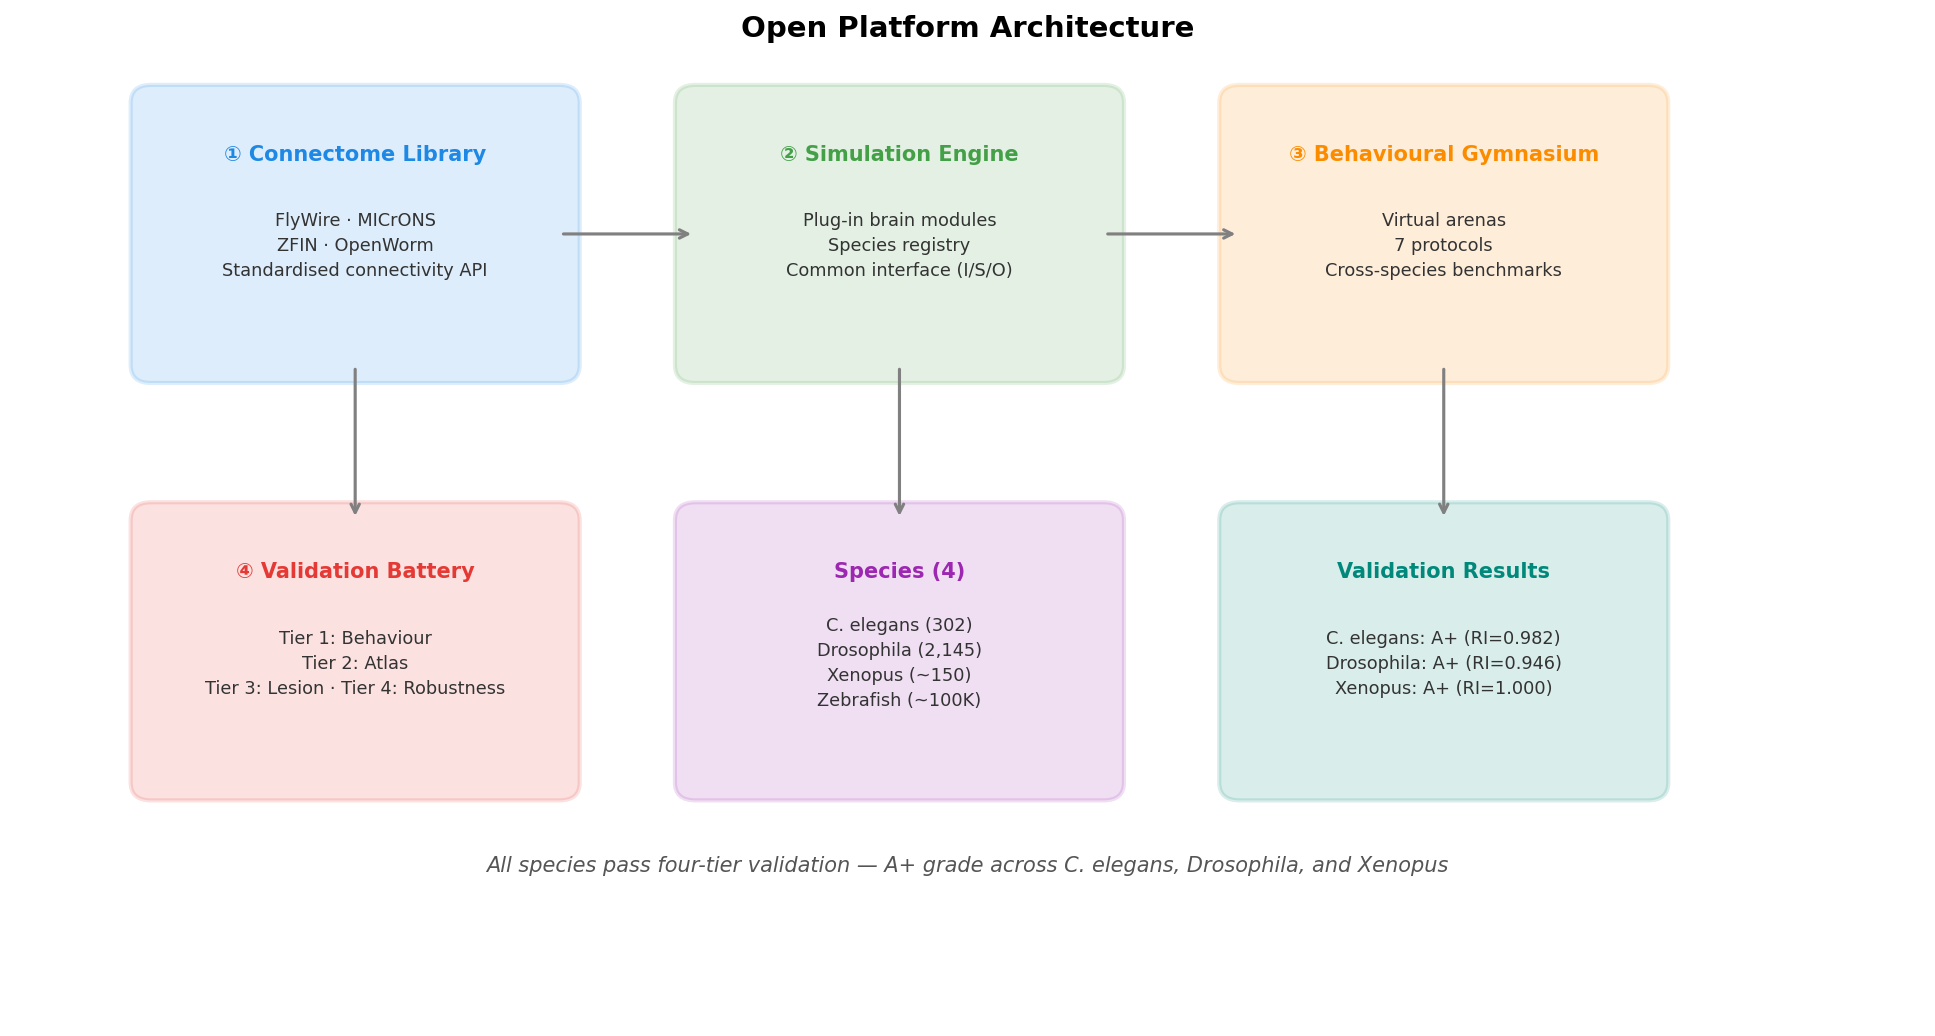
\includegraphics[width=\textwidth]{fig4_platform.png}
  \caption{%
    \textbf{Open platform architecture.}
    Four components support community-wide use of the virtual laboratory
    paradigm.
    \textbf{①~Connectome library}: species-specific connectome databases
    (FlyWire, MICrONS, ZFIN, OpenWorm) are ingested through a
    standardised connectivity API.
    \textbf{②~Modular simulation engine}: plug-in brain region modules
    with a common interface (inputs, state, outputs) are assembled by a
    registry into full-brain avatars; a cerebellar module validated in
    zebrafish can be transplanted into a mouse avatar without
    modification.
    \textbf{③~Behavioural gymnasium}: shared virtual arenas and
    standardised experimental protocols apply identically to any species'
    avatar.
    \textbf{④~Experiment runner}: scripted interventions automatically
    log the full hierarchical state; built-in analytics compute
    correspondence scores against biological reference data.
    A validation feedback loop (dashed arrow, right) allows biological
    benchmark data to update the connectome and module parameters
    iteratively.
    All empirical data sources (bottom row) feed into the platform
    through the connectome library's standardised API.
  }
  \label{fig:platform}
\end{figure}


% ─────────────────────────────────────────────────────────
%  REFERENCES
% ─────────────────────────────────────────────────────────
\clearpage
\section*{References}

\begin{thebibliography}{99}
\setlength{\itemsep}{2pt}

\bibitem{kunst2019}
Kunst, M. et al.
A cellular-resolution atlas of the larval zebrafish brain.
\textit{Neuron} \textbf{103}, 21--38.e5 (2019).

\bibitem{agetsuma2010}
Agetsuma, M. et al.
The habenula is crucial for experience-dependent modification of fear
responses in zebrafish.
\textit{Nat. Neurosci.} \textbf{13}, 1354--1356 (2010).

\bibitem{ahrens2013}
Ahrens, M. B. et al.
Whole-brain functional imaging at cellular resolution using light-sheet
microscopy.
\textit{Nat. Methods} \textbf{10}, 413--420 (2013).

\bibitem{friston2017}
Friston, K. J. et al.
Active inference and epistemic value.
\textit{Cogn. Neurosci.} \textbf{6}, 187--214 (2015).

\bibitem{adams2013}
Adams, R. A., Stephan, K. E., Brown, H. R., Frith, C. D. \&
Friston, K. J.
The computational anatomy of psychosis.
\textit{Front. Psychiatry} \textbf{4}, 47 (2013).

\bibitem{dorkenwald2024}
Dorkenwald, S. et al.
Neuronal wiring diagram of an adult brain.
\textit{Nature} \textbf{634}, 124--138 (2024).

\bibitem{microns2021}
MICrONS Consortium et al.
Functional connectomics spanning multiple areas of mouse visual cortex.
\textit{bioRxiv} https://doi.org/10.1101/2021.07.28.454025 (2021).

\bibitem{bradford2022}
Bradford, Y. M. et al.
Zebrafish information network, the knowledgebase for \textit{Danio rerio}
research.
\textit{Genetics} \textbf{220}, iyac016 (2022).

\bibitem{white1986}
White, J. G., Southgate, E., Thomson, J. N. \& Brenner, S.
The structure of the nervous system of the nematode
\textit{Caenorhabditis elegans}.
\textit{Philos. Trans. R. Soc. Lond. B} \textbf{314}, 1--340 (1986).

\bibitem{payne2018}
Payne, J. L. \& Bhatt, D. L.
OpenWorm: an open-science approach to modelling \textit{Caenorhabditis elegans}.
\textit{Front. Comput. Neurosci.} \textbf{12}, 77 (2018).

\bibitem{markram2015}
Markram, H. et al.
Reconstruction and simulation of neocortical microcircuitry.
\textit{Cell} \textbf{163}, 456--492 (2015).

\bibitem{hines1997}
Hines, M. L. \& Carnevale, N. T.
The NEURON simulation environment.
\textit{Neural Comput.} \textbf{9}, 1179--1209 (1997).

\bibitem{stimberg2019}
Stimberg, M., Brette, R. \& Goodman, D. F. M.
Brian 2, an intuitive and efficient neural simulator.
\textit{eLife} \textbf{8}, e47314 (2019).

\bibitem{sanzleon2013}
Sanz Leon, P. et al.
The Virtual Brain: a simulator of primate brain network dynamics.
\textit{Front. Neuroinform.} \textbf{7}, 10 (2013).

\bibitem{dura2019}
Dura-Bernal, S. et al.
NetPyNE, a tool for data-driven multiscale modelling of brain circuits.
\textit{eLife} \textbf{8}, e44494 (2019).

\end{thebibliography}

% ─────────────────────────────────────────────────────────
%  ACKNOWLEDGEMENTS  (fill before submission)
% ─────────────────────────────────────────────────────────
\section*{Acknowledgements}
The authors thank colleagues at the Brain Korea 21 Project for helpful discussions.
This work was supported by [grant information].

% ─────────────────────────────────────────────────────────
%  AUTHOR CONTRIBUTIONS  (CRediT taxonomy)
% ─────────────────────────────────────────────────────────
\section*{Author Contributions}
J.S.L.: Conceptualization, Methodology, Software, Formal analysis,
Writing---original draft.
H.J.P.: Conceptualization, Supervision, Funding acquisition,
Writing---review \& editing.

% ─────────────────────────────────────────────────────────
%  COMPETING INTERESTS
% ─────────────────────────────────────────────────────────
\section*{Competing Interests}
The authors declare no competing interests.

\end{document}
